%% =============================================================================
%% Mathematische Grundlagen - Grundbegriffe
%% Kapitel 05 - Relationen
%% Autor: Andreas Zeh-Marschke
%% Datum: 2025-03-30
%% =============================================================================

\chapter{Relationen}
\label{cha:Gdl-K05-Relationen}

%% -----------------------------------------------------------------------------
%\begin{unit}
Zu einem der fundamentalen Begriffen der Mathematik gehört der Begriff der
\textbf{Relation}, der im Abschnitt \ref{sec:Relationen:Grundlagen} 
grundlegend definiert wird. Den Relationen liegt das kartesische Produkt von 
Mengen zugrunde. Relationen beschreiben Beziehungen zwischen Elementen von 
Mengen. Die \textbf{Eigenschaften} von Relationen werden anschließend 
(Abschnitt \ref{sec:Relationen:Eigenschaften}) definiert.

Relationen finden sich auch in vielen Bereichen des täglichen Lebens, zum 
Beispiel in den Beziehungen zwischen Menschen: \enquote{Andreas \emph{ist
befreundet mit} Bernd}, \enquote{Claudia \emph{ist verheiratet mit} Dieter}
und \enquote{Ernst \emph{ist Vater von} Franz}. Auch die Stücklistenstruktur
\enquote{ist Teil von} ist eine Relation. Relationen finden auch in der 
Informatik eine wichtige Anwendung. Ein \emph{relationales
Datenbankmodell} basiert auf Relationen. Diese Beispiele sollen nur
andeuten, dass der Begriff der Relationen oft vorkommt.

Zwei wichtige Typen von Relationen, die genauer betrachtet werden, sind die 
\textbf{Äquivalenzrelation} (Abschnitt 
\ref{sec:Relationen:Aequivalenzrelationen}) und die \textbf{Ordnungsrelation}
(Abschnitt \ref{sec:Relationen:Ordnungsrelationen}).
%\end{unit}

%%------------------------------------------------------------------------------

%%------------------------------------------------------------------------------
%% Abschnitt: Grundlagen
%%------------------------------------------------------------------------------
\section{Grundlagen}
\label{sec:Relationen:Grundlagen}

%% -----------------------------------------------------------------------------
\begin{Unit}[Definition Relation]
Die Definition einer Relation ist sehr einfach.

\begin{Definition}
  Es seien $X_1, X_2, \ldots , X_n$ beliebige nicht leere Mengen, dann heißt 
  jede Teilmenge $\mathcal{R} \subseteq X_1 \times X_2 \times \cdots \times 
  X_n$ des kartesischen Produktes eine \textbf{n-stellige Relation}
  \index{Relation} der Mengen $X_1, X_2, \ldots , X_n$. \\
  Zwei Relationen heißen \Begriff{gleich}, wenn sie als Mengen gleich sind.
\end{Definition}
\Translation{Relation}{relation}
\Translation{gleich}{equal}

Die 1-stelligen Relationen einer Menge sind genau die Teilmengen der Menge. 
Als 0-stellige Relationen werden die Elemente der Menge aufgefasst. Eine 
2-stellige Relation heißt auch \Begriff{binäre Relation}\index{Relation, 
binär}.
\Translation{binäre Relation}{binary relation}
\end{Unit}

%% -----------------------------------------------------------------------------
\begin{Unit}[Beispiel]
Zur Verdeutlichung der Definition einige Beispiele von Relationen.

Es seien $X = \{1, 2, 3\}$ und $Y = \{a, b\}$. Daraus ergeben sich für das 
kartesische Produkte $X \times Y$ 
\begin{align}
  X \times Y = \{ (1,a), (1,b), (2,a), (2,b), (3,a), (3,b) \} \ .
\end{align}
Durch $\mathcal{R} := \{ (1,a), (2,b), (3,a), (3,b) \}$ ist eine Relation 
definiert, die mittels einer Tabelle (siehe Tabelle
\ref{tbl:rel:Darstellung Relation in Tabellenform}) oder einer Grafik 
(siehe Abbildung \ref{abb:rel:Darstellung Relation als Grafik}) beschrieben 
werden kann.

\begin{table}[htbp]
\begin{center}
  \begin{tabular}{|c|c|c|c|} \hline
      & 1 & 2 & 3 \\ \hline
    a & X &   & X \\ \hline
    b &   & X & X \\ \hline
  \end{tabular}
  \caption{Darstellung Relation in Tabellenform}
  \label{tbl:rel:Darstellung Relation in Tabellenform}
\end{center}
\end{table}

\begin{figure}[htbp]
\begin{center}
  \setlength{\unitlength}{1.0cm}
  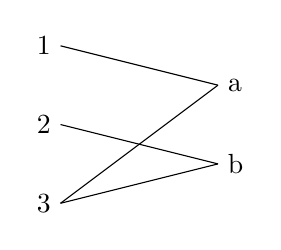
\begin{tikzpicture}[scale=1.0]
    \draw (1.0,1.0) node[left]{3};
    \draw (1.0,2.0) node[left]{2};
    \draw (1.0,3.0) node[left]{1};
    \draw (3.0,1.5) node[right]{b};
    \draw (3.0,2.5) node[right]{a};
    \draw (1.0,3.0) -- (3.0,2.5);
    \draw (1.0,2.0) -- (3.0,1.5);
    \draw (1.0,1.0) -- (3.0,2.5);
    \draw (1.0,1.0) -- (3.0,1.5);
  \end{tikzpicture}
  \caption{Darstellung Relation als Grafik}
  \label{abb:rel:Darstellung Relation als Grafik}
\end{center}
\end{figure}
\end{Unit}

%% -----------------------------------------------------------------------------
\begin{Unit}[Beispiel] 
  Es seien $P = \{p_1, p_2, p_3, p_4\}$ eine Menge von Produkten und $L = 
  \{l_1, l_2, l_3\}$ eine Menge von Lieferanten. Dann ist $P \times L$ das
  kartesische Produkt der Produkte und Lieferanten. Wenn der Lieferant $l_1$ 
  die Produkte $p_1$ und $p_2$, der Lieferant $l_2$ die Produkte $p_1, p_3$ 
  und $p_4$ und der Lieferant $l_3$ die Produkte $p_2$ und $p_4$ liefert, so 
  kann die Relation $\mathcal{R}$ \enquote{wird geliefert von} dargestellt 
  werden durch 
  \begin{align}
    \mathcal{R} = \{(p_1,l_1), (p_2,l_1), (p_1,l_2), (p_3,l_2), (p_4,l_2), 
      (p_2,l_3), (p_4,l_3)\}
  \end{align}
\end{Unit}

%% -----------------------------------------------------------------------------
\begin{Unit}[Beispiel]
  Es sei $M = \{A,B,C,D\}$ eine Menge von vier Orten. Die Relation 
  $\mathcal{R}$ der \emph{Ortsverbindungen} auf $M$ sei definiert durch die
  Eigenschaft, dass das Tupel $(X,Y)$ genau dann in der Relation enthalten 
  ist, wenn es eine Verbindung vom Ort $X$ zum Ort $Y$ gibt. Existiert eine 
  direkte Verbindung von Ort $X$ nach Ort $Y$, dann bedeutet das nicht, dass 
  es auch eine direkte Verbindung von Ort $Y$ zum Ort $X$ gibt. Es sei
  \begin{align}
    \mathcal{R} = \{ &(A,B), (B,A), (A,C), (C,D), \\
      & (D,A), (B,D), (D,B), (B,C), (C,B) \} \nonumber \ . 
  \end{align}
  Die Relation kann auch als Grafik dargestellt werden (siehe Abbildung
  \ref{abb:rel:Ortsverbindungen}). Hierbei wird durch einen gerichteten Pfeil 
  von $X$ nach $Y$ dargestellt, dass das Tupel $(X,Y)$ in der Relation ist, 
  dass   es somit eine direkte Verbindung von $X$ nach $Y$ gibt.

\begin{figure}[htbp]
\begin{center}
  \setlength{\unitlength}{1.0cm}
  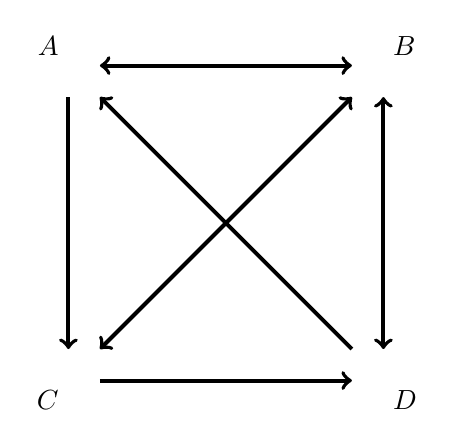
\begin{tikzpicture}[scale=2.0]
    \draw(1.0,3.0) node[above left]{$A$};
    \draw(3.0,3.0) node[above right]{$B$};
    \draw(1.0,1.0) node[below left]{$C$};
    \draw(3.0,1.0) node[below right]{$D$};
    \draw[line width=0.05cm, ->] (1.2,1.0) -- (2.8,1.0);
    \draw[line width=0.05cm, ->] (1.0,2.8) -- (1.0,1.2);
    \draw[line width=0.05cm, <->] (1.2,3.0) -- (2.8,3.0);
    \draw[line width=0.05cm, <->] (3.0,1.2) -- (3.0,2.8);
    \draw[line width=0.05cm, <->] (1.2,1.2) -- (2.8,2.8);
    \draw[line width=0.05cm, ->] (2.8,1.2) -- (1.2,2.8);
  \end{tikzpicture}
  \caption{Beispiel: Ortsverbindungen}
  \label{abb:rel:Ortsverbindungen}
\end{center}
\end{figure}
\end{Unit}

%% -----------------------------------------------------------------------------
\begin{Unit}[Beispiel] 
  Es sei $X = Y = \mg{R}$, dann ist
  \begin{align}
    K_2 := \{(x,y) \in \RR^2 \mid  (x^2\ +\ y^2\ =\ 4) \} 
  \end{align}
  eine Relation von $\RR^2$. Grafisch sind es die Punkte im 2-dimensionalen 
  Anschaungsraum, die auf einem Kreis mit Radius 2 um den Ursprung liegen.
\end{Unit}

%% -----------------------------------------------------------------------------
\begin{Unit}[Beispiel] 
  Es sei $X = Y = \NN$, dann sind
  \begin{align}
    \mathcal{R} := \{ (x,y) \in \NN^2 \mid (x \leq y) \}
  \end{align}
  und
  \begin{align}
    \mathcal{R} := \{ (x,y) \in \NN^2 \mid (x < y) \}
  \end{align}
  Relationen von $\NN^2$. Veranschaulichen Sie sich die Menge grafisch.
\end{Unit}

%% -----------------------------------------------------------------------------
\begin{Unit}[Beispiel] 
  Es sei $X = Y = \NN$, dann ist
  \begin{align}
    \mathcal{R}  := \{ (x,y) \in \NN^2 \mid (x - y = 1) \lor
      (y - x = 1) \} 
  \end{align} eine Relation von $\NN^2$.
\end{Unit}

%% -----------------------------------------------------------------------------
\begin{Unit}[Beispiel] 
  Es sei $M$ eine beliebige Menge und $X = Y = \mathcal{P}(M)$ die Potenzmenge 
  von $M$, dann ist
  \begin{align}
    T := \{ (U,V) \mid (U \subseteq M) \land (V \subseteq M) \land (U \subseteq 
      V) \} 
  \end{align}
  eine Relation von $\mathcal{P}(M)^2$.
\end{Unit}

%% -----------------------------------------------------------------------------
\begin{Unit}[Beispiel] 
  Es sei $X = Y = \ZZ$, dann ist für $n \in \NN$ 
  \begin{align}
    \mathcal{R}_n := \{ (x,y) \in \ZZ^2 \mid n|(x - y) \} 
  \end{align}
  eine Relation von $\ZZ^2$. Ein Tupel $(x,y)$ ist in der Relation, wenn die 
  Differenz der beiden Zahlen durch $n$ teilbar ist. 
  
  Für $n = 1$ ist $\mathcal{R}_1 = \ZZ^2$, also trivial. 
  
  Für $n = 2$ ist $\mathcal{R}_2$ die Menge der ganzzahligen 2-Tupel, für 
  welche die Differenz der beiden Zahlen durch 2 teilbar ist. So sind die 
  Tupel $(0,0)$, $(0,2)$, $(1,3)$, $(12,-6)$ Elemente der Relation, während 
  $(17,12)$ nicht zur Relation gehört. 
  
  Für $n = 5$ sind beispielsweise die Tupel $(0,0)$, $(0,5)$, $(0,10)$, 
  $(1,6)$, $(2,7)$, $(3,8)$, $(5,0)$ und $(17,12)$ in der Relation. Nicht in 
  der Relation sind beispielsweise $(0,1)$, $(0,2)$, $(0,3)$, $(0,4)$ und 
  $(12,8)$.

  Verdeutlichen Sie sich, welche Elemente in der Relation
  \begin{align}
    \mathcal{R}_n = \{ (x,y) \in \ZZ^2 \mid n|(x - y) \}
  \end{align}
  für $n = 1, 2, 3, 4, 5$ und $6$ enthalten sind.
\end{Unit}

%% -----------------------------------------------------------------------------
\begin{Unit}[Definition Inverse Relation]
Für die Relationen können einige spezielle Operationen definiert werden. Eine
davon ist die inverse Relation.

\begin{Definition}
  Es sei $\mathcal{R} \subseteq X \times Y$ eine binäre Relation.
  Die \Begriff{inverse Relation}\index{Relation, inverse}
  $\mathcal{R}^{-1}$ ist definiert durch
  \begin{align}
    \mathcal{R}^{-1} = \{ (y,x) \in Y \times X \mid (x,y) \in \mathcal{R} \} 
    \ .
  \end{align}
\end{Definition}

Ist $(x,y)$ eine Element aus $\mathcal{R} \subseteq X \times Y$, dann ist 
$(y,x)$ ein Element aus $\mathcal{R}^{-1} \subseteq Y \times X$.
\end{Unit}
\Translation{inverse Relation}{inverse relation}

%% -----------------------------------------------------------------------------
\begin{Unit}[Beispiel][Inverse Relation]
  Es sei $X = Y = \NN$ und $\mathcal{R} \subseteq X \times Y = \NN^2$. 
  Hierbei   sei $\mathcal{R}$ definiert durch
  \begin{align}
    \mathcal{R} = \{ (1,1), (1,2), (1,4), (2,3), (4,2)\} \ . 
  \end{align}
  Dann gilt
  \begin{align}
    \mathcal{R}^{-1} = \{ (1,1), (2,1), (4,1), (3,2), (2,4)\} \ . 
  \end{align}
\end{Unit}

%% -----------------------------------------------------------------------------
\begin{Unit}[Definition Komposition]
Eine weitere Operation ist die Komposition von Relationen.

\begin{Definition}
  Es seien $\mathcal{R} \subseteq X \times Y$ und $\mathcal{S} \subseteq Y 
  \times Z$ binäre Relationen. Die \Begriff{Komposition} $\mathcal{S} \circ 
  \mathcal{R}$ ist eine Relation zwischen $X$ und $Z$. Sie ist definiert 
  durch
  \begin{align}
    \mathcal{S} \circ \mathcal{R} = \{ (x,z) \in X \times Z \mid \exists y 
    \in Y : (x,y) \in \mathcal{R} \land (y,z) \in \mathcal{S} \} 
  \end{align}
\end{Definition}

Die Komposition $\mathcal{S} \circ \mathcal{R}$ beinhaltet somit die Tupel 
$(x,z) \in X \times Z$, für die es ein Element $y \in Y$ gibt, so dass sowohl 
$(x,y) \in \mathcal{R}$, als auch $(y,z) \in \mathcal{S}$ gelten. Die 
Schreibweise $\mathcal{S} \circ \mathcal{R}$ ist nicht einheitlich. Manchmal,
auch in früheren Versionen des Skripts, wurde es anders herum geschrieben.
\end{Unit}
\Translation{Komposition}{composition}

%% -----------------------------------------------------------------------------
\begin{Unit}[Beispiel Komposition]
  Es sei $X = Y = Z = \NN$, $\mathcal{R} \subseteq X \times Y = \NN^2$ und 
  $\mathcal{S} \subseteq Y \times Z = \NN^2$. Hierbei sei $\mathcal{R}$
  definiert durch
  \begin{align}
    \mathcal{R} = \{ (1,1), (1,2), (1,4), (2,3), (4,2)\}  
  \end{align}
  und $\mathcal{S}$ durch
  \begin{align}
    \mathcal{S} = \{ (1,3), (2,2), (1,4), (3,5)\} \ .  
  \end{align}
  Dann gilt
  \begin{align}
    \mathcal{S} \circ \mathcal{R} = \{ (1,3), (1,4), (1,2), (2,5), (4,2)\}
  \end{align} 
\end{Unit}

%% -----------------------------------------------------------------------------
\begin{Unit}[Beispiel Komposition]
  Es sei $X = Y = \NN$, $\mathcal{R} \subseteq X \times Y = \NN^2$. Hierbei 
  sei $\mathcal{R}$ definiert durch
  \begin{align}
    \mathcal{R} = \{ (1,1), (1,2), (1,4), (2,3), (4,2)\} \ .
  \end{align}
  Dann gilt
  \begin{align}
    \mathcal{R}^2 &= \mathcal{R} \circ \mathcal{R} = \{ (1,1), (1,2), (1,3), 
    (1,4), (4,3)\} \\
    \mathcal{R}^3 &= \mathcal{R}^2 \circ \mathcal{R} = \{ (1,1), (1,2), 
    (1,3), (1,4) \}
  \end{align} 
  Weiterhin gilt, hier im speziellen Fall, $\mathcal{R}^4$ = $\mathcal{R}^3$.
\end{Unit}

%%------------------------------------------------------------------------------

%%------------------------------------------------------------------------------
%% Abschnitt: Eigenschaften
%%------------------------------------------------------------------------------
\section{Eigenschaften}
\label{sec:Relationen:Eigenschaften}

%% -----------------------------------------------------------------------------
\begin{unit}
Für 2-stellige Relationen $\mathcal{R} \subseteq X \times Y$, mit beliebigen 
nicht leeren Mengen $X$ und $Y$ wird auch $x\mathcal{R}y$ statt $(x,y) \in
\mathcal{R}$ geschrieben. Im nachfolgenden werden hauptsächlich 2-stellige 
Relationen $\mathcal{R} \subseteq X \times X$, mit einer beliebigen Menge 
$X$, betrachtet. Es heißt dann auch Relation \textbf{auf} $X$
\index{Relation auf}. Im Nachfolgenden einige wichtige Eigenschaften von 
Relationen auf $X$.
\end{unit}

%% -----------------------------------------------------------------------------
\begin{Unit}[Definition reflexiv, irreflexiv]
Zuerst werden Beziehungen eines Elementes zu sich selbst betrachtet.
\begin{Definition}
  Es sei $X$ eine beliebige, nicht leere Menge. Eine Relation $\mathcal{R} 
  \subseteq X \times X$ heißt \Begriff{reflexiv}, falls für alle $x \in 
  X$, $(x, x) \in \mathcal{R}$
  \begin{align}
    \forall x \in X:\ (x, x) \in \mathcal{R}
  \end{align}
  gilt. Eine Relation $\mathcal{R} \subseteq X \times X$ heißt 
  \Begriff{irreflexiv}, falls für alle $x \in X$, $(x, x) \notin 
  \mathcal{R}$
  \begin{align}
    \forall x \in X:\ (x, x) \notin \mathcal{R}
  \end{align}
  gilt. 
\end{Definition}

Ist die Relation reflexiv, dann steht jedes Element in einer Beziehung zu sich
selbst. Ist die Relation irreflexiv, dann steht jedes Element nicht in einer
Beziehung zu sich.
\end{Unit}
\Translation{reflexiv}{reflexive}
\Translation{irreflexiv}{irreflexive}

%% -----------------------------------------------------------------------------
\begin{Unit}[Definition symmetrisch, asymmetrisch, antisymmetrisch]
Beziehun\-gen zwischen zwei Elemeneten werden nun betrachtet.
\begin{Definition}
  Es sei $X$ eine beliebige, nicht leere Menge. Eine Relation $\mathcal{R} 
  \subseteq X \times X$ heißt \Begriff{symmetrisch}, falls für alle 
  $x, y \in X$ aus $(x, y) \in \mathcal{R}$ folgt, dass auch $(y, x) \in 
  \mathcal{R}$ 
  \begin{align}
    \forall (x,y \in X)\ :\ (x, y) \in \mathcal{R} \rightarrow (y, x) \in 
      \mathcal{R}
  \end{align}
  gilt. Eine Relation $\mathcal{R} \subseteq X \times X$ heißt 
  \Begriff{asymmetrisch}, falls für alle $x, y \in X$ aus $(x, y) \in 
  \mathcal{R}$ folgt, dass $(y, x) \notin \mathcal{R}$
  \begin{align}
    \forall (x,y \in X)\ :\ (x, y) \in \mathcal{R} \rightarrow (y, x) \notin 
      \mathcal{R}
  \end{align} 
  gilt. Eine Relation $\mathcal{R} \subseteq X \times X$ heißt 
  \Begriff{antisymmetrisch}, falls für alle $x, y \in X$ aus $(x, y) \in 
  \mathcal{R}$ und $(y, x) \in \mathcal{R}$ folgt, dass dann $x\ =\ y$
  \begin{align}
    \forall (x, y \in X)\ :\ (x, y) \in \mathcal{R} \land (y, x) \in 
      \mathcal{R} \rightarrow\ (x = y)
  \end{align}
  gilt.
\end{Definition}
Wenn das Tupel $(x,y)$ in der Relation ist, dann ist das Tupel $(y,x)$ in der 
Relation, wenn die Relation symmetrisch ist. Bei einer asymmetrischen Relation
ist das Tupel $(y,x)$ nicht in der Relation. Bei einer antisymmetrischen 
Relation folgt aus der Tatsache, dass sowohl das Tupel $(x,y)$, als auch das 
Tupel $(y,x)$ in der Relation ist, dass dann $x$ und $y$ gleich sind.

Besonders zu beachten ist, dass die Eigenschaften symmetrisch und 
antisymmetrisch nicht die \enquote{Negation} zueinander sind. Das heißt eine
Relation die nicht symmetrisch ist, ist damit nicht automatisch
antisymmetrisch. Und eine Relation, die nicht antisymmetrisch ist, ist
nicht automatisch damit symmetrisch. Ebenso wenig ist eine Relation, die
nicht symmetrisch ist, asymmetrisch.
\end{Unit}
\Translation{symmetrisch}{symmetric}
\Translation{asymmetrisch}{asymmetric}
\Translation{antisymmetrisch}{antisymmetric}

%% -----------------------------------------------------------------------------
\begin{Unit}[Definition transitiv]
Nun wird eine Folge von Tupeln betrachtet.
\begin{Definition}
  Es sei $X$ eine beliebige, nicht leere Menge. Eine Relation $\mathcal{R} 
  \subseteq X \times X$ heißt \Begriff{transitiv}, falls für alle $x, y, z 
  \in X$ aus $(x, y) \in \mathcal{R}$ und $(y, z) \in \mathcal{R}$ folgt, 
  dass auch $(x, z) \in \mathcal{R}$ gilt:
  \begin{align}
    \forall (x, y, z \in X):\ (x, y) \in \mathcal{R} \land (y, z) \in
      \mathcal{R} \rightarrow\ (x, z) \in \mathcal{R}
  \end{align}
  gilt.
\end{Definition}
Wenn $(x,y)$ und $(y,z)$ aus der Relation sind, dann ist auch $(x,z)$ aus 
der Relation.
\end{Unit}
\Translation{transitiv}{transitive}

%% -----------------------------------------------------------------------------
\begin{Unit}[Definition vollständig, linear, konnex]
Ist es immer möglich, eine Beziehung zwischen zwei Elementen zu haben?
\begin{Definition}
  Es sei $X$ eine beliebige, nicht leere Menge. Eine Relation $\mathcal{R} 
  \subseteq X \times X$ heißt \Begriff{vollständig} oder 
  \Begriff{linear}, falls für alle $x, y \in X$ $(x, y) \in \mathcal{R}$ 
  oder $(y, x) \in \mathcal{R}$ gilt:
  \begin{align}
    \forall (x \in X)\ and\ (y \in X):\ (x, y) \in \mathcal{R} \lor (y, x)
      \in \mathcal{R} \ .
  \end{align}
  Sie heißt \Begriff{konnex}, wenn für alle $x, y \in X$ mit $x \not= y$ 
  gilt, dass $(x, y) \in \mathcal{R}$ oder $(y, x) \in \mathcal{R}$:
  \begin{align}
    \forall (x \in X)\ and\ (y \in X):\ x \not= y \Rightarrow (x, y) \in 
    \mathcal{R} \lor (y, x) \in \mathcal{R} \ .
  \end{align}
\end{Definition}
Mindestens eines der Paare $(x,y)$ und $(y,x)$ ist in der Relation. Wenn eine 
Relation vollständig ist, dann bedeutet dies, dass zu zwei Elementen $x$ und 
$y$ stets $(x,y)$ oder $(y,x)$ (oder auch beide) in der Relation sind.
\end{Unit}
\Translation{vollständig}{complete}
\Translation{linear}{linear}
\Translation{konnex}{connected}

%% -----------------------------------------------------------------------------
\begin{Unit}[Beispiel] 
  Es sei $X = Y = \NN$, dann ist $\mathcal{R} := \{ (x,y) \mid x \leq y) \}$ 
  eine Relation von $\NN^2$. Die Relation ist reflexiv, antisymmetrisch, 
  transitiv und vollständig.
\end{Unit}

%% -----------------------------------------------------------------------------
\begin{Unit}[Beispiel] 
  Es sei $X = Y = \NN$, dann ist $\mathcal{R} := \{ (x,y) \mid x < y) \}$ 
  eine   Relation von $\NN^2$. Die Relation ist irreflexiv, transitiv und 
  antisymmetrisch, jedoch nicht reflexiv oder symmetrisch.
\end{Unit}

%% -----------------------------------------------------------------------------
\begin{Unit}[Beispiel] 
  Es sei $X = Y = \RR$, dann ist $\mathcal{R} := \{ (x,y) \mid x \leq y) \}$ 
  eine Relation von $\RR^2$. Die Relation ist reflexiv, antisymmetrisch, 
  transitiv und vollständig.
\end{Unit}

%% -----------------------------------------------------------------------------
\begin{Unit}[Beispiel] 
  Es sei $X = Y = \RR$, dann ist $\mathcal{R} := \{ (x,y) \mid x^2 + y^2 = 4 \}$ 
  eine Relation von $\RR^2$. Die Relation ist symmetrisch.
\end{Unit}

%% -----------------------------------------------------------------------------
\begin{Unit}[Beispiel] 
  Es seien $X = Y = \ZZ$ und $n \in \NN$, dann ist $\mathcal{R} := \{ (x,y) \mid 
    n|(x - y) \}$ eine Relation von $\ZZ^2$. Die Relation ist reflexiv, 
    symmetrisch und transitiv.
\end{Unit}

%% -----------------------------------------------------------------------------
\begin{Unit}[Definition Äquivalenzrelation, Ordnungsrelation]
Die wichtigsten Relationen erfüllen gleichzeitig mehrere der Eigenschaften 
reflexiv, symmetrisch, antisymmetrisch, transitiv und voll\-stän\-dig.

\begin{Definition}
  Es seien $X$ eine beliebige, nicht leere Menge und $\mathcal{R} \subseteq X 
  \times X$ eine Relation auf $X$.
  \begin{enumerate}
    \item $\mathcal{R}$ heißt \Begriff{Äquivalenzrelation} auf $X$, falls
      sie reflexiv, transitiv und symmetrisch ist. In diesem Fall wird 
      $a \approx b$ anstelle von $(a, b) \in \mathcal{R}$ geschrieben und 
      \enquote{a ist äquivalent zu b} gesagt. 
    \item $\mathcal{R}$ heißt \Begriff{Ordnungsrelation} auf $X$, falls sie 
      reflexiv, transitiv und antisymmetrisch ist. In diesem Fall wird 
      $a \preceq b$ anstelle von $(a, b) \in \mathcal{R}$geschrieben und 
      \enquote{a ist kleiner gleich b} gesagt. 
    \item $\mathcal{R}$ heißt \Begriff{Präferenzrelation} auf $X$, falls 
      sie reflexiv, transitiv und voll\-ständig ist. In diesem Fall wird 
      $a \preceq b$ anstelle von $(a, b) \in \mathcal{R}$ geschrieben und 
      \enquote{a ist höchstens so gut wie b} gesagt.
  \end{enumerate}
\end{Definition}

Bevor die Äquivalenz- und Ordnungsrelationen genauer betrachten werden 
folgen nun einige Beispiele für solche Relationen.
\end{Unit}
\Translation{Äquivalenzrelation}{equivalence relation}
\Translation{Ordnungsrelation}{order relation}
\Translation{Präferenzrelation}{preference relation}

%% -----------------------------------------------------------------------------
\begin{Unit}[Beispiel] 
  Es sei $X = Y = \NN$, dann ist $\mathcal{R}_{\leq} := \{ (x,y) \mid x 
  \leq y) \}$ eine Relation von $\NN^2$. Die Relation ist reflexiv, 
  antisymmetrisch, transitiv und vollständig und daher eine (vollständige)
  Ordnungsrelation (auf $\NN$).
\end{Unit}

%% -----------------------------------------------------------------------------
\begin{Unit}[Beispiel] 
  Es sei $X = Y = \RR$, dann ist $\mathcal{R}_{\leq} := \{ (x,y) \mid x 
  \leq y) \}$ eine Relation von $\RR$. Die Relation ist reflexiv, 
  antisymmetrisch, transitiv und vollständig und daher eine (vollständige)
  Ordnungsrelation (auf $\RR$).
\end{Unit}

%% -----------------------------------------------------------------------------
\begin{Unit}[Beispiel] 
  Es sei $M$ eine beliebige, nicht leere Menge und $X = Y = \mathcal{P}(M)$ 
  die Potenzmenge von $M$, dann ist $\mathcal{R} := \{ (U,V) \mid 
  (U \subseteq V)\}$ eine Relation auf $\mathcal{P}(M)$. Die Relation ist 
  reflexiv, antisymmetrisch und transitiv und daher eine Ordnungsrelation 
  (auf $\mathcal{P}(M)$). Die  Relation ist jedoch nicht vollständig.
\end{Unit}

%% -----------------------------------------------------------------------------
\begin{Unit}[Beispiel] 
  Es sei $X = \RR$, dann wird durch $\mathcal{R} := \{ (x,y) \in \RR^2 
  \mid |x| \leq |y| \}$ eine Präferenzrelation auf $\RR$ definiert. Sie ist
  reflexiv, transitiv und vollständig, jedoch weder symmetrisch noch
  antisymmetrisch, daher ist es eine Präferenzrelation.
\end{Unit}

%% -----------------------------------------------------------------------------
\begin{Unit}[Beispiel] 
  Es sei $X$ eine Menge von Gütern. Jedem $x \in X$ sei ein Wert $u(x)$ 
  zugeordnet, der als Nutzen von $x$ interpretiert wird. Dann wird durch 
  $\mathcal{R} := \{ (x,y) \in X^2 \mid u(x) \leq u(y) \}$ eine
  Präferenzrelation auf $X$ definiert. Sie ist reflexiv, transitiv und 
  vollständig, jedoch weder symmetrisch noch antisymmetrisch, daher ist es 
  eine Präferenzrelation.
\end{Unit}

%%------------------------------------------------------------------------------
%% Abschnitt: Äquivalenzrelationen
%%------------------------------------------------------------------------------
\section{Äquivalenzrelationen}
\label{sec:Relationen:Aequivalenzrelationen}

%% -----------------------------------------------------------------------------
\begin{Unit}[Beispiel]
Eine Äquivalenzrelation ist eine Relation, die reflexiv, symmetrisch und 
transitiv ist. Dazu einige Beispiele.

\begin{enumerate}
\item 
  In der Geometrie ist die Parallelität von Geraden eine Äquivalenzralation 
  auf der Menge der Geraden.
\item
  Die Anzahl der Elemente einer Menge (Mächtigkeit) ist eine 
  Äquivalenzrelation auf der Menge der endlichen Mengen.
\end{enumerate}
\end{Unit}

%% -----------------------------------------------------------------------------
\begin{Unit}[Beispiel] 
  Es sei $X = \ZZ$, dann ist für $n \in \NN \backslash \{1\}$
  \begin{align}
    \mathcal{R}_n := \{ (x,y) \mid  (n|(x - y) \} \subseteq\ \ZZ^2
  \end{align}
  eine Relation. Die Relation ist reflexiv, symmetrisch und transitiv, daher 
  ist die Relation eine Äquivalenzrelation. Ist $(x, y) \in \mathcal{R}_n$ 
  dann wird auch $x \equiv y \modulo n$ oder $x \equiv_n y$ geschrieben und 
  \enquote{$x$ ist kongruent zu $y$ modulo $n$} gesagt. \\
  Sind $x$ und $y$ kongruent modulo $n$, dann besitzen $x$ und $y$ bei der 
  Division durch $n$ den selben Rest.

Für $n = 1$ wäre $\mathcal{R}_1 = \ZZ^2$. Daher ist dieses Beispiel einfach 
und wird im weiteren nicht vertieft.
\end{Unit}

%% -----------------------------------------------------------------------------
\begin{Unit}[Beispiel]
  Es sei $X = \NN$. Jedem $n \in \NN$ wird durch $q(n)$ die Quersumme 
  zugeordnet. Durch
  \begin{align}
    \mathcal{R} := \{ (x,y) \in \NN^2 \mid q(x) = q(y) \}
  \end{align}
  ist eine Äquivalenzrelation auf $\NN$ definiert wird.
\end{Unit}

%% -----------------------------------------------------------------------------
\begin{Unit}[Definition Äquivalenzklasse]
Die Elemente einer Menge, die bezüglich einer Äquivalenzrelation zueinander 
äquivalent sind bilden eine Teilmenge der Menge. Diese Teilmengen werden nun
genauer betrachtet.

\begin{Definition}
  Es sei $X$ eine beliebige Menge und $\mathcal{R} \subseteq X \times X$ eine 
  Äquivalenzrelation auf $X$. Für jedes $x \in X$ heißt die Menge
  \begin{align}
    [x] := \{ y \in X \mid y \approx x \}
  \end{align}
  die \Begriff{Äquivalenzklasse} von $x$.
\end{Definition}

Eine Äquivalenzrelation $[x]$ enthält somit all diejenigen Elemente der Menge, 
die zu $x$ äquivalent sind.
\end{Unit}
\Translation{Äquivalenzrelation}{equivalence relation}

%% -----------------------------------------------------------------------------
\begin{Unit}[Bemerkung]
Für Äquivalenzklassen gelten folgende Aussagen:

\begin{Bemerkung}
  Es sei $X$ eine beliebige Menge und $\mathcal{R} \subseteq X \times X$ eine 
  Äquivalenzrelation auf $X$, dann gelten:
  \begin{enumerate}
    \item Jede Äquivalenzklasse ist ungleich der leeren Menge. 
    \item Sind zwei Elemente $x$ und $y$ äquivalent, dann sind die 
      Äquivalenzklassen $[x]$ und $[y]$ von $x$ und $y$ identisch. 
    \item Jedes Element gehört zu genau einer Äquivalenzklasse.
    \item Je zwei Äquivalenzklassen sind entweder identisch oder disjunkt.
  \end{enumerate}
\end{Bemerkung}

Beweis:
\begin{enumerate}
  \item Da $x \in [x]$ gilt, ist eine Äquivalenzklasse nicht die leere Menge.
  \item Wenn $x \approx y$ gilt, dann gilt für ein $z \in X$:
    \begin{align}
      z \in [x] \leftrightarrow z \approx x \leftrightarrow z \approx y 
      \leftrightarrow z \in [y]
    \end{align}
    Die mittlere (Aussagen-)Äquivalenz gilt auf Grund der Transitivität der 
    Relation, da $x \approx y$ gilt. Damit wurde die Mengenidentität von 
    $[x]$ und $[y]$ gezeigt, da jedes Element von $[x]$ auch Element von 
    $[y]$ ist und umgekehrt. Also wurde die gegenseitige Teilmengenbeziehung
    gezeigt.
  \item Da $x \in [x]$, gehört $x$ mindestens zu einer Äquivalenzklasse. 
    Falls $x \in [y]$ und $x \in [z]$ gelten, dann folgt daraus, dass 
    $x \approx y$ und $x \approx z$ gilt. Auf Grund der Transitivität der 
    Relation ist dann $y \approx z$ und somit $[y] = [z]$. Damit gehört x zu 
    maximal einer und zu genau einer Äquivalenzklasse.
  \item Folgt direkt aus den obigen Aussagen.
\end{enumerate}\qed
\end{Unit}

%% -----------------------------------------------------------------------------
\begin{Unit}[Anmerkung]
Jede Äquivalenzrelation auf einer Menge $X$ zerlegt damit $X$ in paarweise
disjunkte, nicht leere Mengen, die Äquivalenzklassen. Es entsteht somit eine 
Klasseneinteilung. Genauso folgt aus einer Klasseneinteilung einer Menge eine 
Äquivalenzrelation, indem zwei Elemente genau dann in einer Äquivalenzklasse 
sind, wenn sie zur selben Klasse bezüglich der Klasseneinteilung gehören.
\end{Unit}

%% -----------------------------------------------------------------------------
\begin{Unit}[Definition Quotientenmenge]
Eine Äquivalenzrelation erzeugt eine neue Menge, die Menge der 
Äquivalenzklassen von $X$. Hierbei muss beachtet werden, dass die Elemente 
der Klasseneinteilung selber Mengen sind, nämlich die Äquivalenzklassen.

\begin{Definition}
  Es sei $X$ eine beliebige, nicht leere Menge und $\mathcal{R} \subseteq X 
  \times X$ eine Äquivalenzrelation auf $X$, dann heißt die Menge der
  Äquivalenzklassen von $X$ nach $\mathcal{R}$
  \begin{align}
    X / \mathcal{R} := \{ [x] \mid x \in X \}
  \end{align}
  die \Begriff{Quotientenmenge} von $X$ nach $\mathcal{R}$.\\
  Ein Element $y \in [x]$ heißt \Begriff{Repräsentant} der Klasse $[x]$.\\
  Eine Menge $V$ heißt \Begriff{vollständiges Repräsentantensystem}\index
  {Repräsentantensystem} von $X / \mathcal{R}$, wenn $V$ genau ein Element aus 
  jeder Klasse von $X / \mathcal{R}$ enthält.
\end{Definition}
\end{Unit}
\Translation{Quotientenmenge}{quotient set}
\Translation{Repräsentantensystem}{system of representatives}

%% -----------------------------------------------------------------------------
\begin{Unit}[Beispiel] 
  Die Geraden mit paralleler Richtung bilden die Äquivalenzklassen. Die 
  Parallelität von Geraden führt zum Begriff der Richtung.
\end{Unit}

%% -----------------------------------------------------------------------------
\begin{Unit}[Beispiel] 
  Die Mengen mit gleicher Elementanzahl bilden die Äquivalenzklassen auf der 
  Menge der endlichen Mengen. Die Mächtigkeit von Mengen führt zum Begriff 
  der Kardinalität.
\end{Unit}

%% -----------------------------------------------------------------------------
\begin{Unit}[Beispiel]
  Für jedes $n \in \NN\backslash \{1\}$ ist
  \begin{align}
    \mathcal{R}_n := \{ (x,y) \mid n|(x-y) \} \subseteq \ZZ^2
  \end{align}
  eine Relation. Ist $(x,y) \in \mathcal{R}_n$ dann wird auch $x \equiv y 
  \modulo n$ geschrieben und \enquote{$x$ ist kongruent zu $y$ modulo $n$} 
  gesagt. Für $n \in \NN \backslash \{1\}$ gibt es $n$ Repräsentanten der
  Quotientenmenge $\ZZ /
  \mathcal{R}_n$. Die Klassen seien $[0], [1], \ldots, [n-1]$. 
  Die Repräsentanten seien $0, 1, \ldots, n-1$. Durch
  \begin{align}
    [x] + [y]\ :=\ [x + y]
  \end{align}
  und
  \begin{align}
    [x] \cdot [y]\ := [x \cdot y]
  \end{align}
  wird auf der Quotientenmenge $\ZZ / \mathcal{R}_n  =:  \ZZ_n$ eine Addition 
  und eine Multiplikation definiert.
  \begin{enumerate}
    \item $\mathcal{R}_n$ ist eine Äquivalenzrelation.
    \item Für beliebiges $n \in \NN\backslash\{1\}$ und $i=0,1,\ldots,n-1$ 
    gilt
      \begin{align}
        [i] = \{z \in \ZZ \mid \exists x \in \ZZ : z = xn + i \}
      \end{align}
  \end{enumerate}
\end{Unit}

%% -----------------------------------------------------------------------------
\begin{Unit}[Beispiel]
  Es sei $M = \NN \times \NN$ die Menge der 2-Tupel mit natürlichen Zahlen. 
  Eine Relation $\mathcal{R}\ \subseteq M \times M$ sei definiert durch:
  \begin{align}
    \left( (a,b)\;,\;(c,d) \right) \in \mathcal{R}\ :\Leftrightarrow
      (a + d = b + c) \ .
  \end{align}
  Statt $\left( (a,b)\;,\;(c,d) \right) \in \mathcal{R}$ wird auch 
  $(a,b) \sim (c,d)$ geschrieben. 

  $\mathcal{R}$ ist eine Äquivalenzrelation auf $M = \NN \times \NN$. Die 
  Quotientenmenge $(\NN \times \NN) / \mathcal{R}$ oder $(\NN \times \NN) / 
  \sim$ ist äquivalent zu den ganzen Zahlen $\ZZ$.
\end{Unit}

%%------------------------------------------------------------------------------
%% Abschnitt: Ordnungsrelationen
%%------------------------------------------------------------------------------
\section{Ordnungsrelationen}
\label{sec:Relationen:Ordnungsrelationen}

%% -----------------------------------------------------------------------------
\begin{Unit}[Definition][teilweise geordnet, streng geordnet]
Es seien $M$ eine Menge und $\mathcal{R} \subseteq M \times M$ eine 
Ordnungsrelation. Eine Relation ist eine Ordnungsrelation, wenn sie reflexiv, 
transitiv und antisymmetrisch ist. Statt $(x,y) \in \mathcal{R}$ wird 
$x \preceq y$ geschrieben und \enquote{x ist kleiner (oder gleich) y} gesagt.

Wichtige Begriffe für Ordnungsrelationen werden eingeführt.

\begin{Definition}
  Eine binäre Relation $\preceq$ auf einer Menge $M$ heißt \Begriff
  {Ordnungsrelation}, \Begriff{teilweise Ordnung}\index{Ordnung, teilweise} 
  oder \Begriff{partielle Ordnung}\index{Ordnung, partielle}, wenn sie 
  reflexiv, antisymmetrisch und transitiv ist. Die Menge $M$ heißt dann 
  \Begriff{geordnete Menge}\index{Menge, geordnet} $(M,\preceq)$ oder 
  \Begriff{teilweise geordnete Menge}\index{Menge,teilweise geordnet}.\\
  Wenn eine Relation transitiv, jedoch nicht reflexiv ist, dann heißt die 
  Relation eine \Begriff{strenge Ordnungsrelation}\index{Ordnungsrelation, 
  strenge}. Eine Menge mit einer strengen Ordnungsrelation heißt \Begriff
  {streng geordnete Menge}\index{Menge, streng geordnet}.
\end{Definition}
\Translation{Ordnungsrelation}{partially ordered relation}
\Translation{partielle Ordnung}{partial order}
\Translation{strenge Ordnungsrelation}{strict partially order relation}
\Translation{streng geordnet}{strict partial order}

Für ein teilweise geordnete Menge wird auch kurz \Begriff
{tgo Menge}\index{Menge, tgo} oder \Begriff{poset} \enquote{partially 
ordered set} geschrieben.
\end{Unit}

%% -----------------------------------------------------------------------------
\begin{Unit}[Anmerkung]
Es sei $M$ eine Menge. Ist $\mathcal{R} \subseteq M \times M$ eine 
Ordnungsrelation, so kann daraus eine strenge Ordnungsrelation gebildet 
werden, indem die Relation $\mathcal{R} \backslash \mathcal{D} \subseteq 
M \times M$ gebildet wird, mit $\mathcal{D} := \{(x,x) \mid x \in M\}$. Es 
wird somit die \enquote{Diagonale} der Menge $M$ entfernt. Auf der anderen 
Seite kann aus einer strengen Ordnungsrelation eine Ordnungsrelation gebildet
werden, indem diese \enquote{Diagonale} zur Relation hinzugefügt wird. Daher 
wird zwischen einer Ordnungsrelation und einer strengen Ordnungsrelation 
hin- und herschalten.
\end{Unit}

%% -----------------------------------------------------------------------------
\begin{Unit}[Beispiel] 
  Die Mengen $(\NN, \leq)$, $(\ZZ, \leq)$, $(\QQ, \leq)$ und $(\RR, \leq)$ 
  mit der bekannten kleiner-gleich-Beziehung sind geordnete Mengen. \\
  Die Mengen $(\NN, <)$, $(\ZZ, <)$, $(\QQ, <)$, $(\RR, <)$ sind streng 
  geordnete Mengen.
\end{Unit}

%% -----------------------------------------------------------------------------
\begin{Unit}[Beispiel] 
  Es sei $M$ eine Menge, dann ist $(\mathcal{P}(M), \subseteq)$ eine geordnete 
  Menge. $(\mathcal{P}(M), \subset)$ ist eine streng geordnete Menge.
\end{Unit}

%% -----------------------------------------------------------------------------
\begin{Unit}[Beispiel] 
  Die Menge $(\NN, |)$ mit der Ordnungsrelation
  \begin{align}
    x \preceq y : \Leftrightarrow\ x|y
  \end{align}
  ist eine geordnete Menge. \\
  In diesem Beispiel ist die Ordnungsrelation durch die Teilbarkeit der 
  Zahlen bestimmt.
\end{Unit}

%% -----------------------------------------------------------------------------
\begin{Unit}[Beispiel]
  Für alle $n \in \NN$ gilt, dass $n|n$ gilt, daher ist die Relation reflexiv. 
  Es seien $n,m \in \NN$. Wenn $n|m$ und $m|n$ gilt, dann folgt daraus 
  $n = m$, somit ist die Relation antisymmetrisch. Wenn für $n,m,l \in \NN$ 
  gilt: $n|m$ und $m|l$, dann gilt auch $n|l$, und daher ist die Relation 
  transitiv. Somit ist die Relation insgesamt eine Ordnungsrelation.
\end{Unit}

%% -----------------------------------------------------------------------------
\begin{Unit}[Definition linear geordnet]
Die reellen Zahlen können auf einem Zahlenstrahl angeordnet werden. Gilt diese
Eigenschaft allgemeiner?

\begin{Definition}
  Eine Ordnungsrelation $\preceq$ auf einer Menge $M$ heißt \Begriff{total 
  geordnet}\index{geordnet, total}, \Begriff{konnex} oder \Begriff
  {linear geordnet}\index{geordnet, linear}, wenn für alle Elemente $x$, $y$ 
  der Menge $M$ $x \preceq y$ oder $y \preceq x$ gilt.
  \begin{align}
    (M, \preceq) \text{ linear geordnet } :\Leftrightarrow \forall 
    (x, y \in M): (x \preceq y) \lor (y \preceq x) \ .
  \end{align}
\end{Definition}
\Translation{linear geordnet}{linear ordered}

Bei einer total geordneten Menge verwendet wird oftmals auch das Symbol 
$\leq$ statt $\preceq$ verwendet. Damit wird die die Nähe zur totalen
Ordnung auf den Zahlenmengen $\NN$, $\ZZ$, $\QQ$ und $\RR$ verdeutlicht.

Bei einer linear geordneten Menge können die Elemente der Menge linear
angeordnet werden. Es kann für zwei Elemente der Menge stets angegeben werden, 
welche von beiden Zahlen kleiner ist.
\end{Unit}

%% -----------------------------------------------------------------------------
\begin{Unit}[Beispiel] 
  $(\NN, \leq)$, $(\ZZ, \leq)$, $(\QQ, \leq)$ und $(\RR, \leq)$ sind linear 
  geordnete Mengen.
\end{Unit}

%% -----------------------------------------------------------------------------
\begin{Unit}[Beispiel] 
  Es sei $M$ eine Menge, dann ist $(\mathcal{P}(M), \subseteq)$ keine linear 
  geordnete Menge.
\end{Unit}

%% -----------------------------------------------------------------------------
\begin{Unit}[Beispiel] 
  $(\NN, |)$ ist keine linear geordnete Menge.
\end{Unit}

%% -----------------------------------------------------------------------------
\begin{Unit}[Definition Ordnungsdiagramme]
Ordnungsstrukturen endlicher Mengen $(M, \preceq)$ lassen sich in einfachen 
Fällen übersichtlich in einem Diagramm darstellen. Diese Diagramme heißen
\Begriff{Ordnungsdiagramm} oder \Begriff{Hasse-Diagramm}, benannt nach 
dem deutschen Mathematiker Helmut Hasse (1898 - 1979)\index[names]{Hasse, 
Helmut}\footnote{\url{https://de.wikipedia.org/wiki/Helmut_Hasse}}. 
Jedem Element der Menge wird ein Punkt der Zeichenebene zugeordnet. Ist $a 
\preceq b$, so wird ein Pfeil von $a$ nach $b$ gezeichnet. Es kann vereinbart 
werden, dass ein Element $b$ oberhalb eines Elements $a$ gezeichnet wird, 
wenn $a \preceq b$ ist. Darüber hinaus werden $a$ und $b$ einfach verbunden. 
Ein Pfeil ist nicht notwendig, da durch die Anordnung \enquote{unten - oben} 
die Pfeilrichtung entnommen werden kann. Um die Anzahl der Linien zu 
reduzieren, werden keine Verbindungen eines Elements mit sich selbst 
gezeichnet, das heißt, dass die reflexive Eigenschaft nicht dargestellt wird.
Darüber hinaus wird $a$ nicht mit $b$ verbunden, wenn $b$ auch über andere 
Punkte mit $a$ verbunden ist, das heißt, die transitive Eigenschaft wird 
nicht dargestellt.
\end{Unit}
\Translation{Ordnungsdiagramm}{Hasse diagram}

%% -----------------------------------------------------------------------------
\begin{Unit}[Beispiel]
  Es sei $M = \{ n \in \NN \mid 1 < n < 10 \}$ und $x \preceq y 
  :\Leftrightarrow x|y$. Dann kann die Ordnungsrelation folgendermaßen 
  grafisch mit Hilfe eines Ordnungs- oder Hasse-Diagramm dargestellt werden 
  (siehe Abbildung \ref{abb:rel:Beispiel: Ordnungsrelation}).

\begin{figure}[htbp]
\begin{center}
  \setlength{\unitlength}{1.0cm}
  \begin{tikzpicture}[scale=1.0]
    \draw (1.0,1.0) node[below]{$2$};
    \draw (1.0,3.0) node[above]{$4$};
    \draw (1.0,5.0) node[above]{$8$};
    \draw (2.0,4.0) node[above]{$6$};
    \draw (3.0,2.0) node[below]{$3$};
    \draw (3.0,5.0) node[above]{$9$};
    \draw (4.5,3.0) node[below]{$5$};
    \draw (6.0,4.0) node[below]{$7$};
    \draw (1.0,1.0) -- (1.0,3.0);
    \draw (1.0,3.8) -- (1.0,5.0);
    \draw (1.0,1.0) -- (2.0,4.0);
    \draw (3.0,2.0) -- (2.0,4.0);
    \draw (3.0,2.0) -- (3.0,5.0);
  \end{tikzpicture}
  \caption{Beispiel: Ordnungsrelation}
  \label{abb:rel:Beispiel: Ordnungsrelation}
\end{center}
\end{figure}
\end{Unit}

%% -----------------------------------------------------------------------------
\begin{Unit}[Beispiel]

\begin{figure}[htbp]
\begin{center}
  \setlength{\unitlength}{1.0cm}
  \begin{tikzpicture}[scale=1.0]
    \draw (1.0,1.0) node[below]{$2$};
    \draw (1.0,3.0) node[above]{$4$};
    \draw (2.0,4.0) node[below]{$6$};
    \draw (2.0,6.0) node[above]{$12$};
    \draw (3.0,2.0) node[below]{$3$};
    \draw (4.5,3.0) node[below]{$5$};
    \draw (4.5,5.0) node[above]{$25$};
    \draw (6.0,4.0) node[below]{$7$};
    \draw (4.5,3.0) -- (4.5,5.0);  % 5 -- 25
    \draw (1.0,1.0) -- (2.0,3.4);  % 2 -- 6
    \draw (1.0,1.0) -- (1.0,3.0);  % 2 -- 4
    \draw (2.0,4.0) -- (2.0,6.0);  % 6 -- 12
    \draw (1.0,3.8) -- (2.0,6.0);  % 4 -- 12
    \draw (3.0,2.0) -- (2.0,3.4);  % 3 -- 6
  \end{tikzpicture}
  \caption{Beispiel: maximale und minimale Elemente}
  \label{abb:rel:Beispiel: maximale und minimale Elemente}
\end{center}
\end{figure}

\label{bsp:Relationen:Ordnungsrelation}
  Es sei $M = \{2, 3, 4, 5, 6, 7, 12, 25\}$ mit der Ordnungsrelation $a \preceq 
  b :\Leftrightarrow a|b$. Das Ordnungsdiagramm hat folgendes Aussehen (siehe 
  Abbildung \ref{abb:rel:Beispiel: maximale und minimale Elemente}) In diesem 
  Beispiel gibt es kein Element, das größer als 12, 25 oder 7 ist. Wird die 
  Menge auf die Element $\{2, 3, 4, 6, 12\}$ eingeschränkt, dann ist die 12 
  sogar größer als jedes andere Element der Menge. Dies führt zu Definitionen 
  von ausgezeichneten Elementen einer geordneten Menge.
\end{Unit}

%% -----------------------------------------------------------------------------
\begin{Unit}[Definition maximales Element, größtes Element]
Die Elemente im vorherigen Beispiel werden nun klar definiert.
  
\begin{Definition}
  Es sei $(M,\preceq)$ eine geordnete Menge. Ein Element $m$ aus $M$ heißt
  \Begriff{maximales Element}\index{Element, maximales} von $M$ ($m = 
  maxEl(M))$, wenn es kein Element gibt, das größer als $m$ ist:
  \begin{align}
    m = maxEl(M) :\Leftrightarrow (m \in M) \land [\forall (x \in M): m 
      \preceq x \rightarrow x = m] \ .
  \end{align} 
  Ein Element $g$ aus $M$ heißt \Begriff{größtes Element}\index{Element, 
  größtes} oder \Begriff{Maximum} von $M$ ($g = grEl(M))$, wenn $g$ größer 
  als jedes andere Element von $M$ ist:
  \begin{align}
    g = grEl(M) :\Leftrightarrow (g \in M) \land \forall (x \in M): 
    x \preceq g \ .
  \end{align} 
\end{Definition}
\Translation{maximales Element}{maximal element}
\Translation{größtes Element}{greatest element}

Für ein maximales Element gibt es keine Elemente in der Menge, die größer 
sind als dieses maximale Element. Ein größtes Element ist größer als jedes 
andere Element. Das ist ein kleiner, aber entscheidender Unterschied, der zu
beachten ist. Eine Menge kann durchaus mehrere maximale Element haben. Wenn 
ein größtes Element existiert, dann ist dieses eindeutig.
\end{Unit}

%% -----------------------------------------------------------------------------
\begin{Unit}[Definition minimales Element, kleinstes Element]
Nun die Elemente, die in der Ordnung unten stehen.
  
\begin{Definition}
  Es sei $(M,\preceq)$ eine geordnete Menge. Ein Element $m$ aus $M$ heißt 
  \Begriff{minimales Element}\index{Element, minimales} von $M$ ($m = 
  minEl(M)$), wenn es kein Element gibt, das kleiner als $m$ ist:
  \begin{align}
    m = minEl(M) :\Leftrightarrow (m \in M) \land [\forall (x \in M): 
    x \preceq m 
      \rightarrow x = m] \ .
  \end{align}
  Ein Element $k$ aus $M$ heißt \Begriff{kleinstes Element}\index{Element, 
  kleinstes} oder \Begriff{Minimum} von $M$ ($k = klEl(M)$), wenn $k$ 
  kleiner als jedes andere Element von $M$ ist:
  \begin{align}
    k = klEl(M) :\Leftrightarrow (k \in M) \land \forall(x \in M): 
    k \preceq x \ .
  \end{align}
\end{Definition}
\Translation{minimales Element}{minimal element}
\Translation{kleinstes Element}{least element}

Für ein minimales Element gibt es keine Elemente in der Menge, die kleiner 
sind als dieses minimale Element. Ein kleinstes Element ist kleiner als 
jedes andere Element. Das ist ein kleiner, aber entscheidender Unterschied, 
der zu beachten ist. Eine Menge kann durchaus mehrere minimale Element haben. 
Wenn ein kleinstes Element existiert, dann ist dieses eindeutig.
\end{Unit}

%% -----------------------------------------------------------------------------
\begin{Unit}[Beispiel] 
  Im Beispiel \ref{bsp:Relationen:Ordnungsrelation} sind 12, 25 und 7 
  maximale Elemente, die Zahlen 2, 3, 5 und 7 sind minimale Elemente. Es gibt 
  kein größtes oder kleinstes Element. Ein Element kann zugleich maximales und
  minimales Element sein. Für die Teilmenge {2, 3, 4, 6, 12} ist 12 ein 
  größtes Element. Ein größtes Element einer Menge muss nicht existieren. Genau
  sowenig ein kleinstes Element.
\end{Unit}

%% -----------------------------------------------------------------------------
\begin{Unit}[Beispiel]
  \label{bsp:Relationen:Wurzel2}
  Es sei
  \begin{align}
    F := \{x \in \QQ \mid x = 1 - \frac{1}{n}, n \in \NN \}
  \end{align}
  eine Teilmenge der geordneten Menge $(\QQ, \leq)$. Alle Elemente der Menge 
  sind kleiner 2 oder auch kleiner 3/2 oder auch kleiner 1. Somit gibt es 
  Element aus der Obermenge $\QQ$ von $F$, die eine obere Schranke für die 
  Elemente der Menge von $F$ bilden.
\end{Unit}

%% -----------------------------------------------------------------------------
\begin{Unit}[Definition Schranke, beschränkt]
Dies führt zu folgenden Definitionen.

\begin{Definition}
  Es sei $(M,\preceq)$ eine geordnete Menge und $T$ eine Teilmenge von $M$ 
  mit   der selben Ordnungsrelation. Ein Element $o$ aus $M$ heißt 
  \Begriff{obere Schranke} von $T$ ($o\ =\ obSch(T)$), wenn alle Elemente von 
  $T$ kleiner oder gleich $o$ sind
  \begin{align}
    o = obSch(T) :\Leftrightarrow  (o \in M) \land \forall (x \in T):
      x \preceq o \ .
  \end{align}
  Existiert eine obere Schranke für eine Menge $T$, so heißt die Menge 
  \Begriff{nach oben beschränkt}\index{beschränkt, nach oben}. \\ 
  Ein Element $u$ aus $M$ heißt \Begriff{untere Schranke}\index{Schranke, 
  untere} von $T$ ($u = untSch(T)$), wenn alle Elemente von $T$ größer oder 
  gleich $u$ sind
  \begin{align}
    u = untSch(T) :\Leftrightarrow (u \in M) \land \forall (x \in T): 
    u \preceq x \ .
  \end{align}
  Existiert eine untere Schranke für eine Menge $T$, so heißt die Menge 
  \Begriff{nach unten beschränkt}\index{beschränkt, nach unten}.
\end{Definition}
\Translation{Schranke}{bound}
\Translation{beschränkt}{bounded}
\Translation{obere Schranke}{upper bound}
\Translation{untereSchranke}{lower bound}

Eine obere oder untere Schranke einer Menge $T$ muss nicht in der Menge $T$ 
selbst enthalten sein, sie können in einer Obermenge existieren. Wenn eine 
Menge $T$ ein größtes oder ein kleinstes Element hat, dann ist dieses Element 
auch zugleich eine obere oder untere Schranke für die Menge $M$.
\end{Unit}

%% -----------------------------------------------------------------------------
\begin{Unit}[Beispiel]
  Für die obige Menge $F$ (siehe Beispiel \ref{bsp:Relationen:Wurzel2}) 
  sei $S$ die Menge der oberen Schranken. Es stellt sich die Frage nach 
  dem kleinsten Element dieser Menge. In diesem Beispiel ist 1 das kleinste 
  Element der oberen Schranken. Die 1 ist nicht in der Menge $F$ enthalten, 
  jedoch in der Obermenge $\QQ$.
\end{Unit}

%% -----------------------------------------------------------------------------
\begin{Unit}[Definition Grenze, Supremum, Infimum]
\ 

\begin{Definition}
  Ein Element $o$ aus $M$ heißt \Begriff{obere Grenze}\index{Grenze, obere} 
  von $T$ ($o = obGr(T)$), wenn $o$ das kleinste Element der Menge der oberen 
  Schranken von $T$ ist. Das Element $o$ heißt dann auch \Begriff{Supremum} 
  von $T$:
  \begin{align}
    o = obGr(T) :\Leftrightarrow (o \in M) \land o = klEl(S) 
  \end{align}
  mit $S = \{s \mid s = obSch(M) \}$.

  Ein Element $u$ aus $M$ heißt \Begriff{untere Grenze}\index{Grenze, 
  untere} von $T$ ($u = untGr(T)$), wenn $u$ das größte Element der Menge der 
  unteren Schranken von $T$ ist. Das Element $u$ heißt dann auch \Begriff
  {Infimum} von $T$:
  \begin{align}
    u = untGr(T) :\Leftrightarrow (u \in M) \land u = grEl(S) 
  \end{align}
  mit $S = \{s \mid s = untSch(M)\}$.
\end{Definition}
\Translation{obere Grenze}{supremum}
\Translation{Supremum}{supremum}
\Translation{untere Grenze}{infimum}
\Translation{Infimum}{infimum}

Eine obere oder untere Grenze muss nicht immer existieren. 
\end{Unit}

%% -----------------------------------------------------------------------------
\begin{Unit}[Beispiel]
  Sei nun
  \begin{align}
    W := \{x \in \QQ \mid x^2 \leq 2 \} \subseteq \QQ \ .
  \end{align}
  Die Menge $W$ ist nach oben beschränkt, denn beispielsweise 2; 1,5 oder 
  1,42 sind obere Schranken. Es gibt jedoch keine obere Grenze von $W$ in 
  $\QQ$, da $\sqrt{2}$ keine rationale Zahl ist. Erst wenn nicht $\QQ$, 
  sondern $\RR$ als Obermenge betrachtet wird, hat die Menge $W$ eine obere 
  Grenze.
\end{Unit}

%% -----------------------------------------------------------------------------
\begin{Unit}[Beispiel]
  Es sei $A := \{t \in \mg{N}\ |\ (t|36)\ and (t < 15)\}$ mit der 
  Ordnungsstruktur, die durch $a \leq b :\Leftrightarrow a|b$ definiert ist. 
  Die Elemente der Menge $A$ sind $A = \{1, 2, 3, 4, 6, 9, 12\}$. Das 
  Ordnungsdiagramm ist in Abbildung 
  \ref{abb:rel:Ordnungsrelation Teiler von 36} zu sehen.

\begin{figure}[htbp]
\begin{center}
  \setlength{\unitlength}{1.0cm}
  \begin{tikzpicture}[scale=1.5]
    \draw (0.50,2.50) node[below]{$4$};
    \draw (1.50,1.50) node[below]{$2$};
    \draw (1.50,3.50) node[below]{$12$};
    \draw (2.50,0.50) node[below]{$1$};
    \draw (2.50,2.50) node[below]{$6$};
    \draw (3.50,1.50) node[below]{$3$};
    \draw (4.50,2.50) node[below]{$9$};
    \draw (1.30,2.90) -- (0.70,2.30);
    \draw (2.30,1.90) -- (1.70,1.30);
    \draw (3.30,0.90) -- (2.70,0.30);
    \draw (4.30,1.90) -- (3.70,1.30);
    \draw (0.70,1.90) -- (1.30,1.30);
    \draw (1.70,0.90) -- (2.30,0.30);
    \draw (1.70,2.90) -- (2.30,2.30);
    \draw (2.70,1.90) -- (3.30,1.30);
  \end{tikzpicture}
  \caption{Ordnungsrelation Teiler von 36}
  \label{abb:rel:Ordnungsrelation Teiler von 36}
\end{center}
\end{figure}

  Die $9$ und die $12$ sind maximale Elemente, denn es gibt keine Elemente in 
  der Menge, die größer sind. Die $6$ hingegen ist kein maximales Element, da 
  die $12$ größer als die $6$ ist. Ein größtes Element existiert nicht, denn die 
  $12$ ist gemäß der Ordnungsstruktur nicht größer als $9$, da die $9$ kein 
  Teiler der $12$ ist. In der Obermenge der natürlichen Zahlen gibt es 
  verschiedene obere Schranken bezüglich der Ordnungsstruktur, zum Beispiel die 
  $36$ oder auch die $72$. Die $18$ ist keine obere Schranke, denn die $12$ ist 
  kein Teiler der $18$, also ist die $18$ nicht größer als jedes Element der 
  Menge. Das Supremum ist die $36$.

  Die $1$ ist minimales Element, kleinstes Element und Infimum der Menge.
\end{Unit}
